\chapter{Modell} \label{chap:dynamics_of_Furuta_pend}

\section{asd}
\begin{align}
	\mathbf q = \begin{bmatrix}
		q_1\\
		q_2
	\end{bmatrix}
	=\begin{bmatrix}
		\varphi	\\
		\theta
	\end{bmatrix}.
\end{align}


\begin{align}
	T = \dfrac{1}{2}\sum_{j=1}^{2} \left( m_j \mathbf v_{C_j}^2 + \bm\omega_j^\mathrm{T} \mathbf J_{j,C_j} \bm\omega_j\right).
	\label{eq:kin_energy}
\end{align}


Egyenlet hivatkozás: a kinetikus energia általánosan a \eqref{eq:kin_energy} egyenlet mutatja.

Irodalmi hivatkozás: \cite{stepan2001vibrations} vagy többet egyzserre \cite{stepan1989retarded,stepan2001vibrations}.

A bifurkációs diagram a \ref{fig:eq_pos_dfi}.~ábrán látható. A\texttt{ASDxxx}x

\begin{figure}[bth]
	\centering
	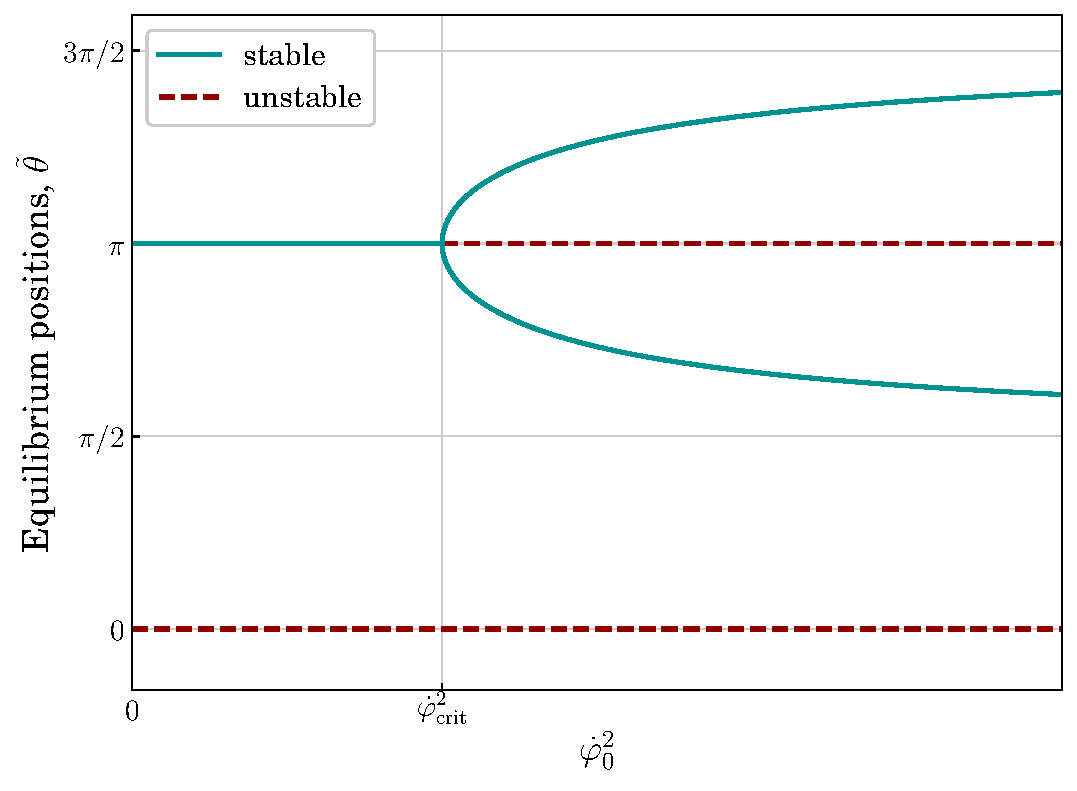
\includegraphics[width=0.9\linewidth]{eq_pos_dfi2.pdf}
	\caption{Bifurcation diagram of equilibrium positions.}
	\label{fig:eq_pos_dfi}
\end{figure}



